\documentclass[a4paper,12pt]{article}

% 页面设置
\usepackage[top=2.54cm, bottom=2.54cm, left=3.17cm, right=3.17cm]{geometry}
\usepackage{fancyhdr}
\usepackage{ctex}
\usepackage{setspace}
\usepackage{graphicx}
\usepackage{times}
\usepackage{float}

% 页眉页脚设置
\pagestyle{fancy}
\fancyhf{}
\fancyhead[C]{\songti\zihao{-5}中央民族大学2026年大学生暑期社会实践成果}
\fancyfoot[C]{\thepage}
\renewcommand{\headrulewidth}{0.4pt}
\setlength{\headheight}{15pt}
\setlength{\headsep}{1.5cm}
\setlength{\footskip}{1.75cm}

% 行距设置 - 固定值22磅
\usepackage{setspace}
\setlength{\baselineskip}{22pt}
\setlength{\lineskip}{0pt}
\setlength{\lineskiplimit}{0pt}

% 字体设置
\setCJKmainfont{SimSun}

% 图片路径
\graphicspath{{./个人报告照片/}}

\begin{document}

% 标题
\begin{center}
\songti\zihao{3}\textbf{铭记烽火 赓续红色初心}
\end{center}
\begin{flushright}
\songti\zihao{3}——中国人民抗日战争纪念馆暑期社会实践报告
\end{flushright}

\vspace{22pt}

% 正文
\songti\zihao{5}
\setlength{\parindent}{2em}
\linespread{1.0}
\selectfont

\section*{\songti\zihao{-3}\textbf{一、实践内容}}

2026年8月20日，我作为"赴北京市丰台区铭记烽火赓续红色初心调研实践团"成员，与安良玉、王冲两位同学一起前往中国人民抗日战争纪念馆开展为期3小时的暑期社会实践活动。作为团队成员，我主要负责第3展区"全民族抗战的中流砥柱——中国共产党的光辉历程"板块的深度调研学习。

在实践过程中，我系统学习了中国共产党在抗日战争中发挥的中流砥柱作用。通过参观展览，我深入了解了九一八事变后中国共产党率先举起武装抗日旗帜的历史，学习了吉鸿昌烈士"恨不抗日死，留作今日羞。国破尚如此，我何惜此头"的爱国情怀，感受了一二九运动中青年学生的爱国热情，认识了八路军第115师平型关大捷的重大意义，领悟了毛泽东《论持久战》的战略智慧，了解了延安作为革命圣地吸引无数爱国青年奔赴的历史，以及国际友人支援中国抗战的感人事迹。

在调研过程中，我认真记录展陈内容，仔细观看历史文物和影像资料，用相机拍摄重要展品和展板，确保全面准确地掌握第一手资料。同时，我也与团队成员保持沟通，共同学习了第5展区抗战胜利与历史启示的内容，对十四年抗战历程有了完整的认识。

\section*{\songti\zihao{-3}\textbf{二、实践成效}}

通过本次实践活动，我在思想认识、知识积累和能力培养等方面都取得了显著成效。

在思想认识方面，我深刻认识到中国共产党的领导是抗战胜利的根本保证。从率先举起抗日旗帜，到制定正确的战略方针，再到开辟敌后战场、领导人民战争，中国共产党始终发挥着中流砥柱作用。这段历史让我更加坚定了听党话、跟党走的信念，增强了对中国特色社会主义的道路自信、理论自信、制度自信和文化自信。

在知识积累方面，我系统掌握了抗日战争特别是敌后战场的历史知识。从九一八事变到七七事变，从局部抗战到全民族抗战，从战略防御到战略相持再到战略反攻，我对十四年抗战的历史脉络有了清晰的认识。特别是通过学习《论持久战》等军事理论著作的展示，我理解了中国共产党人的战略智慧和理论创新能力。

在能力培养方面，我的资料收集能力、文字表达能力和团队协作能力都得到了提升。在调研过程中，我学会了如何快速准确地记录关键信息，如何有条理地整理学习资料，如何与团队成员有效沟通协作。这些实践能力对我今后的学习和工作都具有重要意义。

\section*{\songti\zihao{-3}\textbf{三、实践心得}}

本次实践活动让我深受教育和启发，有以下几点深刻体会。

第一，历史是最好的教科书。只有真正走进历史现场，直面历史文物和史料，才能深刻理解历史的厚重和现实的意义。书本上的知识是抽象的，而纪念馆里的每一件文物、每一张照片、每一段影像都是具体的、鲜活的，它们让我真切感受到革命先烈的英勇牺牲和今天和平生活的来之不易。

第二，青年要担当时代责任。在抗战时期，无数青年学生投笔从戎、奔赴延安，为民族独立和人民解放英勇奋斗。一二九运动中的青年学生，用他们的爱国行动唤醒了民众的抗日意识。这些历史告诉我，青年一代有理想、有本领、有担当，国家就有前途，民族就有希望。在新时代，我们同样要把个人理想融入国家发展，以青春之力担当民族复兴大任。

第三，理论学习与实践体验相结合。通过这次实践，我深刻认识到，理论学习固然重要，但实践体验同样不可或缺。只有将课堂学习与社会实践相结合，才能真正做到知行合一。今后我要积极参加各类社会实践活动，在实践中增长才干、锤炼品格。

第四，团队协作精神至关重要。本次实践活动采用团队协作模式，每个人负责不同的展区，最后汇总形成完整的调研成果。这让我深刻体会到团队协作的重要性。在今后的学习和工作中，我要继续培养团队意识，学会与他人有效沟通、密切配合，共同完成任务。

\section*{\songti\zihao{-3}\textbf{四、实践照片}}

\begin{figure}[H]
\centering
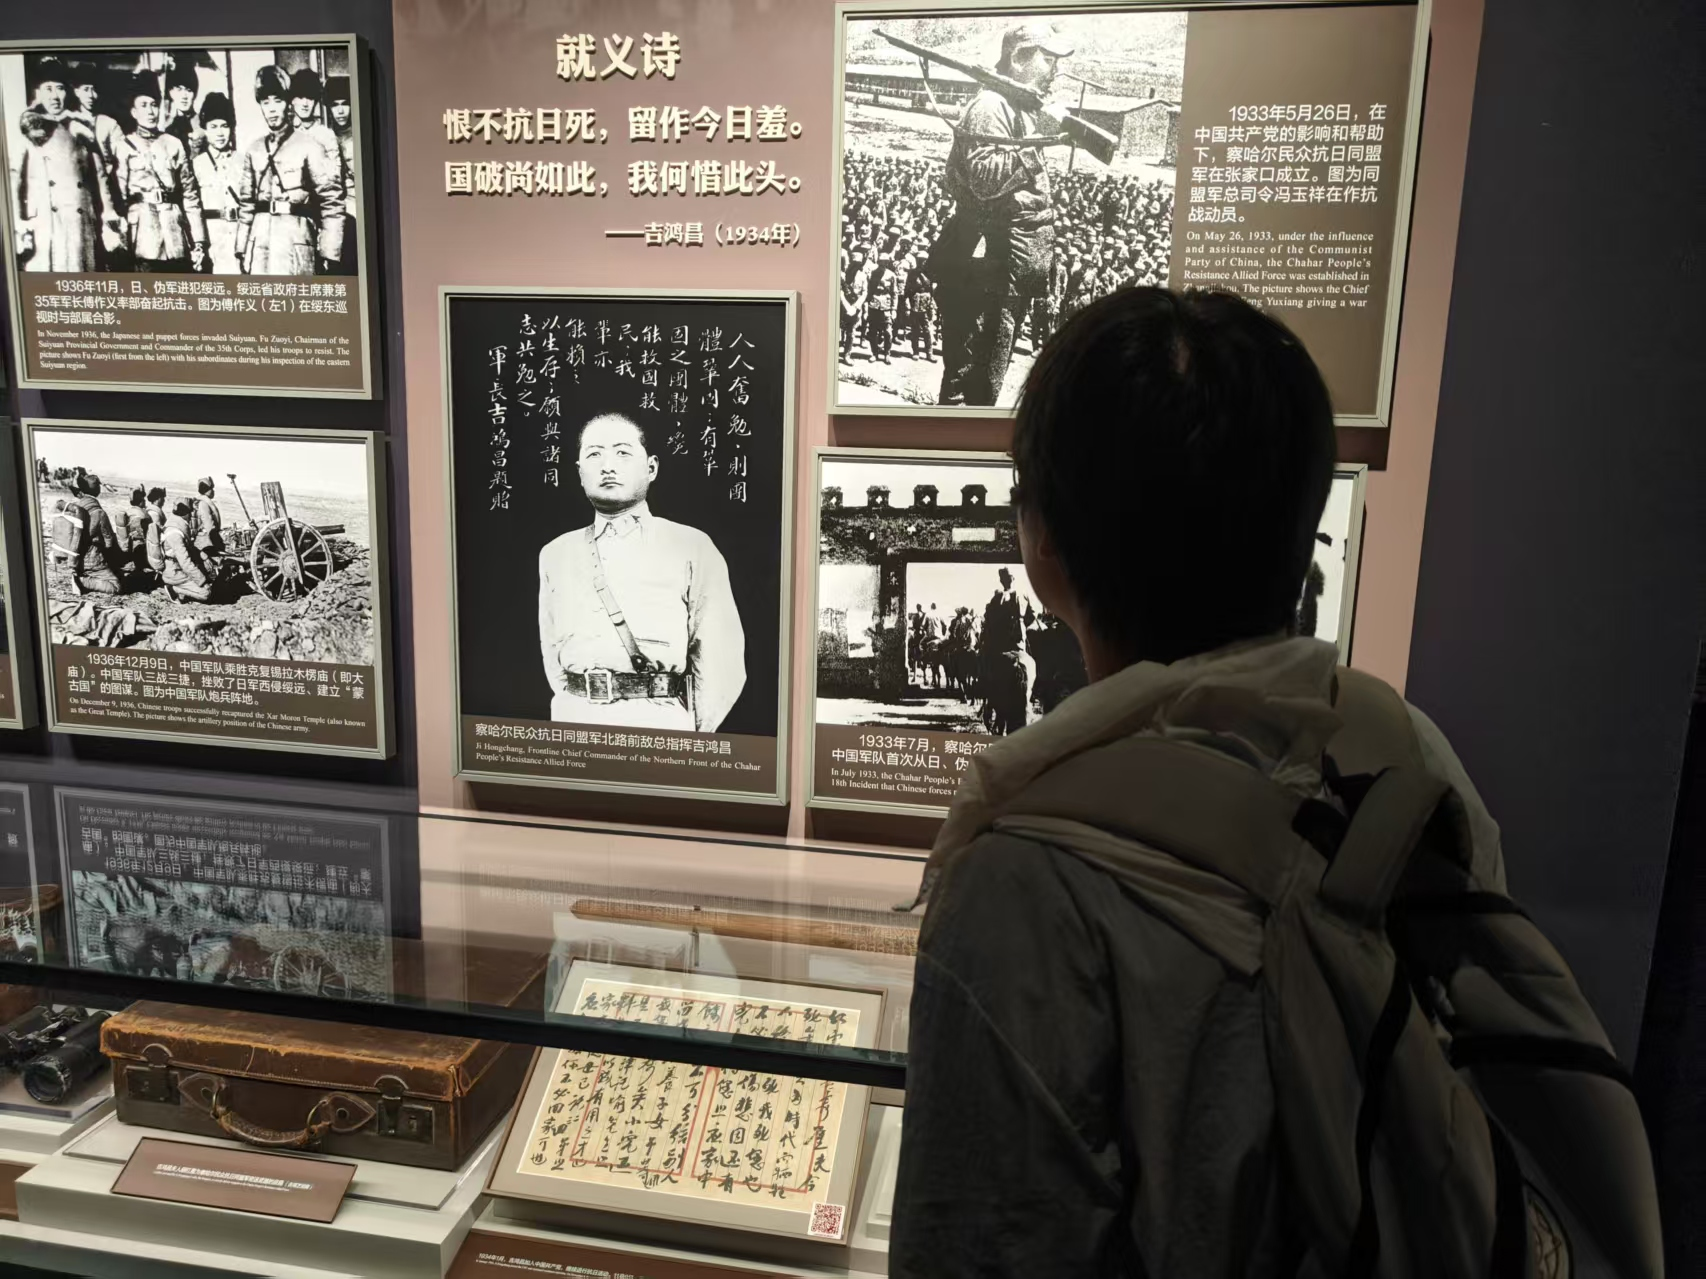
\includegraphics[width=0.6\textwidth]{A (5).jpg}
\caption{参观吉鸿昌烈士史料展区}
\end{figure}

\begin{figure}[H]
\centering
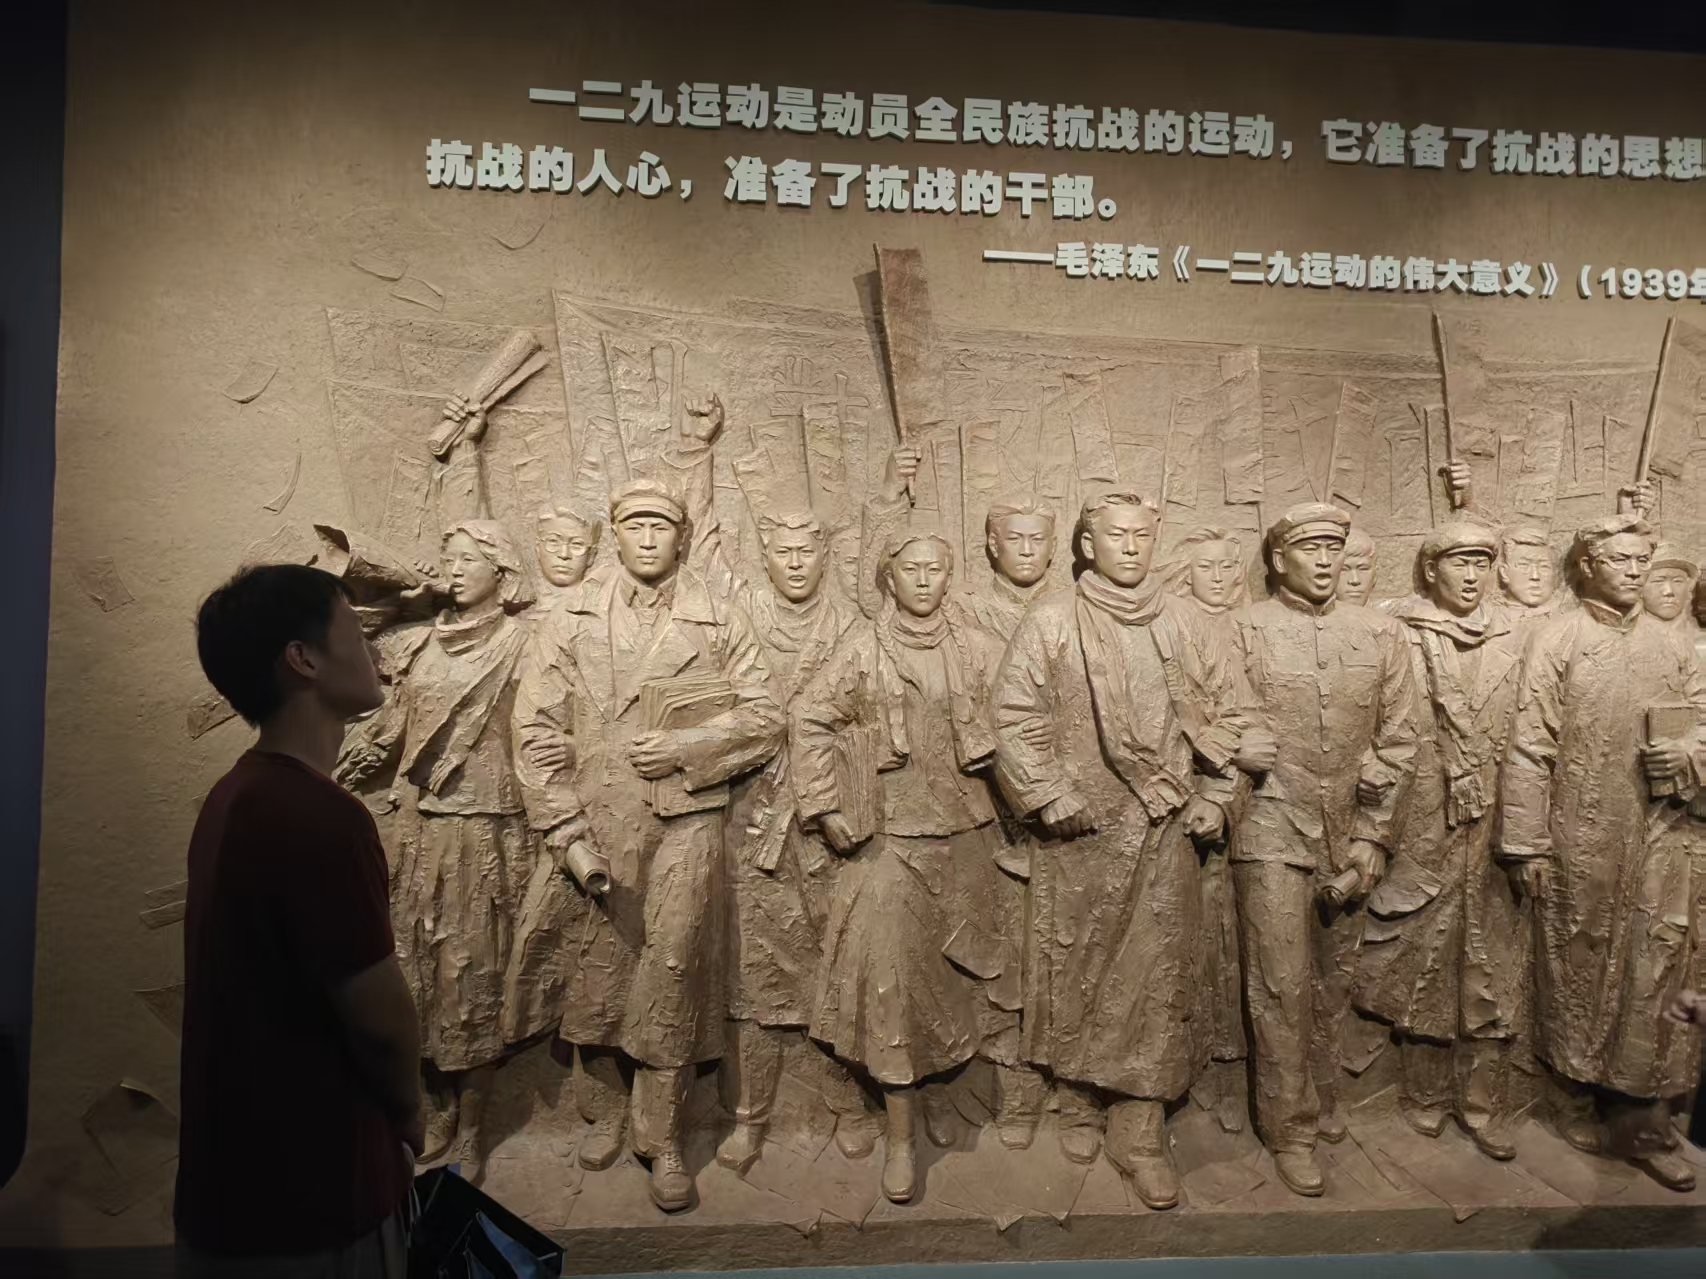
\includegraphics[width=0.6\textwidth]{A (6).jpg}
\caption{学习一二九运动历史}
\end{figure}

\begin{figure}[H]
\centering
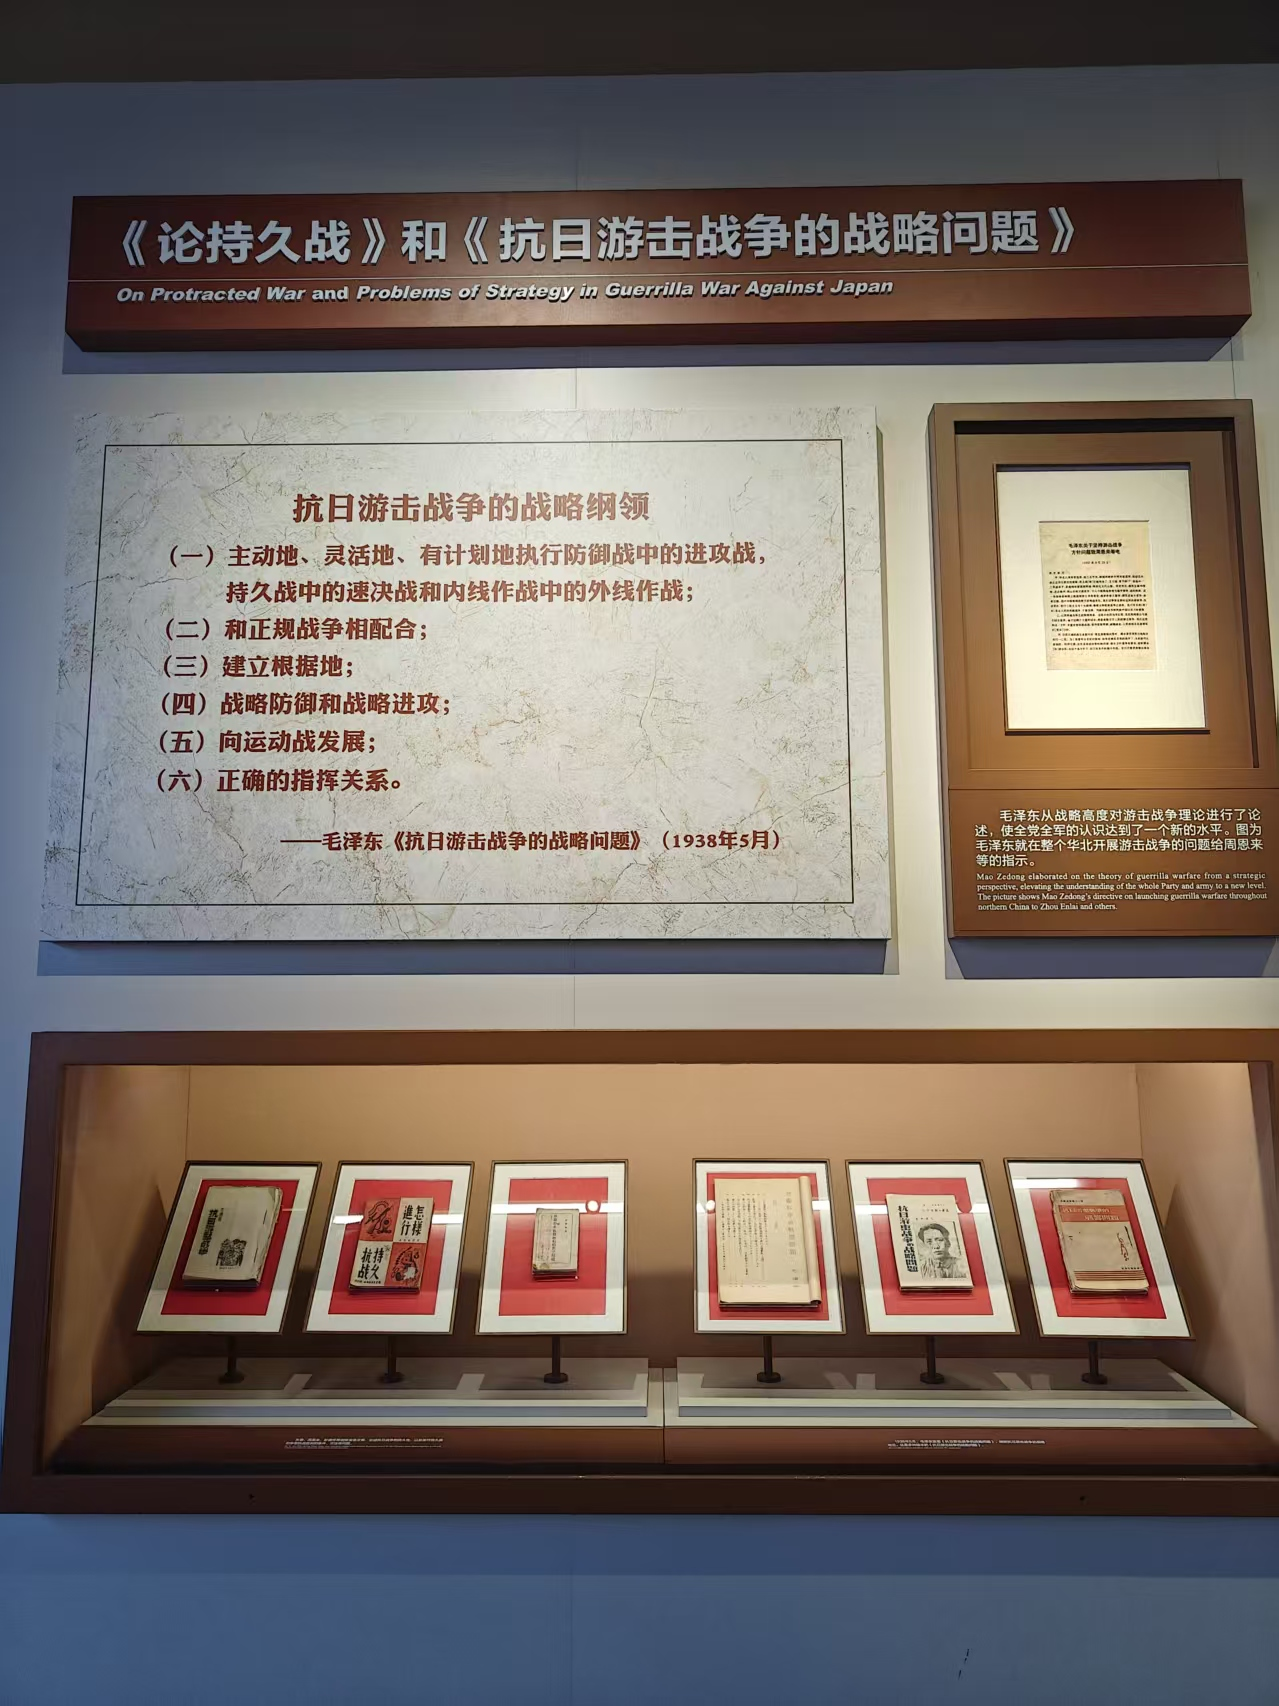
\includegraphics[width=0.6\textwidth]{A (9).jpg}
\caption{学习《论持久战》军事理论}
\end{figure}

\vspace{22pt}

通过本次暑期社会实践活动，我不仅学到了丰富的历史知识，更重要的是接受了一次深刻的爱国主义教育和党史学习教育。铭记历史、缅怀先烈、珍爱和平、开创未来，这是我们青年一代的使命和责任。我将把本次实践的所学所思所悟转化为学习动力，努力提升自己的综合素质，为实现中华民族伟大复兴的中国梦贡献青春力量。

\vspace{22pt}

\begin{flushright}
\songti\zihao{5}
实践人：刘佳鹏\\
实践地点：中国人民抗日战争纪念馆\\
实践时间：2026年8月20日
\end{flushright}

\end{document}
